\documentclass[]{article}
\usepackage[utf8]{inputenc}
\usepackage{fullpage}
\usepackage[pdftex]{graphicx}
\usepackage{hyperref}

\def \GG {grammar of graphics }

\title{
	An introduction to \texttt{ggplot}:\\
 	An implementation of the \GG in R
}
\author{Hadley Wickham}

\date{2006-02-27}

\usepackage{/Library/Frameworks/R.framework/Resources/share/texmf/Sweave}
\begin{document}
\setkeys{Gin}{width=3in} 
%\VignetteIndexEntry{An introduction to ggplot}

\maketitle

\section{Introduction}

Currently, R has two major systems for plotting data, base graphics and lattice graphics \cite{sarkar:2005}.  Base graphics provide low level access to the underlying display, and make it easy to build up a graphic piece-by-piece, and to use multiple data sources.  However, you must take care of the details, such as legends and common axis scales, yourself.  Lattice graphics are high level, and take care of most of the details, but this makes it difficult to incorporate data from multiple sources.  Lattice graphics are an implementation of trellis graphics, as described by Cleveland \cite{cleveland:1993,cleveland:1994}.

The Grammar of Graphics \cite{wilkinson:1999} presents a comprehensive grammar with which to describe graphics.  The key concept is that a graphic is produced by mapping data values to aesthetic attributes of graphical objects (grobs).  For example, a scatterplot maps the values of the $x$ and $y$ variables to the position of the points.  A bubble plot additionally maps the area of the points to a third variable.  Mappings range from simple, e.g. a linear mapping from data value to position on the screen, to complex, e.g. mapping a transformed variable to a colour scale.  These mappings are supplemented by guides, such as legends and axes, to complete the graphic.  The grammar of graphics concentrates on static graphics.  A detailed grammar for interactive and dynamic graphics has yet to be developed, although some efforts have been made in that direction \cite{wilhelm:2005}.

The R package \texttt{ggplot} was developed as a response to the shortcomings of the current plotting systems.  It uses the ideas of the \GG to provide a  new plotting system combining the advantages of both base and lattice graphics.  Conditioning and shared axes are handled automatically, while maintaining the ability to build up a plot step by step from multiple data sources.  It also implements a more sophisticated multidimensional conditioning system and a consistent interface to map data to aesthetic attributes.  It uses the powerful and flexible grid graphics \cite{murrell:2005} extensively.

The following section provides an overview of \texttt{ggplot} and what parts of the \GG have been implemented.  Next I show \texttt{ggplot} in use, and finally, discuss the framework that powers it.

\section{Overview}

The \GG is extensive and the implementation in \texttt{ggplot} is not yet complete.  I have focussed mainly on the ideas of chapters seven and eight, geometry and aesthetics, and the implementation of these is largely complete.  Transformations, split in the \GG into variable, scale and coordinate transformations, have been combined into one system.  This makes the implementation somewhat less flexible, but considerably easier to program.  

In general, \texttt{ggplot} is less rigid, and less comprehensive, than the \GG.  This makes it more suitable for use in a situation where there is less control over the data.   For example, in \texttt{ggplot} you can use data from multiple sources without explicitly specifying how the data sets are linked together.  In practice, for static graphics, it turns out that this is a good compromise: it makes it very easy to combine data from multiple sources, and the linking information that you lose is not necessary for static plots.  We can be less comprehensive in \texttt{ggplot} because it is not a stand-alone application: we have the full capabilities of R available.

\section{Example}

This example introduces \texttt{ggplot} through the analysis of the \texttt{tips} data set, which is data about the tips collected by a waiter over the course of several months.  You can find out more about the data set with \texttt{?tips}. This example is included in the \texttt{ggplot} package, and you can run it using \texttt{example(ggplot)} or \texttt{vignette("introduction", "ggplot")}.

Unlike base and lattice graphics, with \texttt{ggplot} you explicitly build up a plot object.  This makes it much easier to deal with multiple versions of the same plot, easily experimenting with different display options, and rolling-back to previous versions.

The first step is to create a new plot object.  This is where we specify the defaults that control how the plot appears.  The first (and most important) argument is the default data frame.  We also specify a default set of aesthetic mappings.  Here we map the $y$ position to the $tip$, and the $x$ position to the $total\_bill$.  These defaults are used when we add graphical objects (grobs) to the plot.  

\begin{Schunk}
\begin{Sinput}
> library(ggplot)
\end{Sinput}
\end{Schunk}
\begin{Schunk}
\begin{Sinput}
> p <- ggplot(tips, aesthetic = list(y = tip, x = total_bill))
\end{Sinput}
\end{Schunk}

Next we add grobs to the display.  A grob (a graphical object) determines the type of plot that is created.  For example, a scatterplot is made up of point grobs, and a barchart is made up of bar grobs.  To add grobs, we use \texttt{ggXXX} functions.  The arguments to these functions are a plot object, a list of aesthetic mappings, other parameters and a dataset (if you don't want to use the default).  There are many different grob functions to choose from: points, lines, bars, areas, histograms, box plots, contours, and so on.  You can see a full list in \texttt{?ggplot}.   

Here we add points to create a scatterplot.  Since we haven't explicitly specified a data set or aesthetic mappings, \texttt{ggpoint} uses the defaults stored in the plot object.  

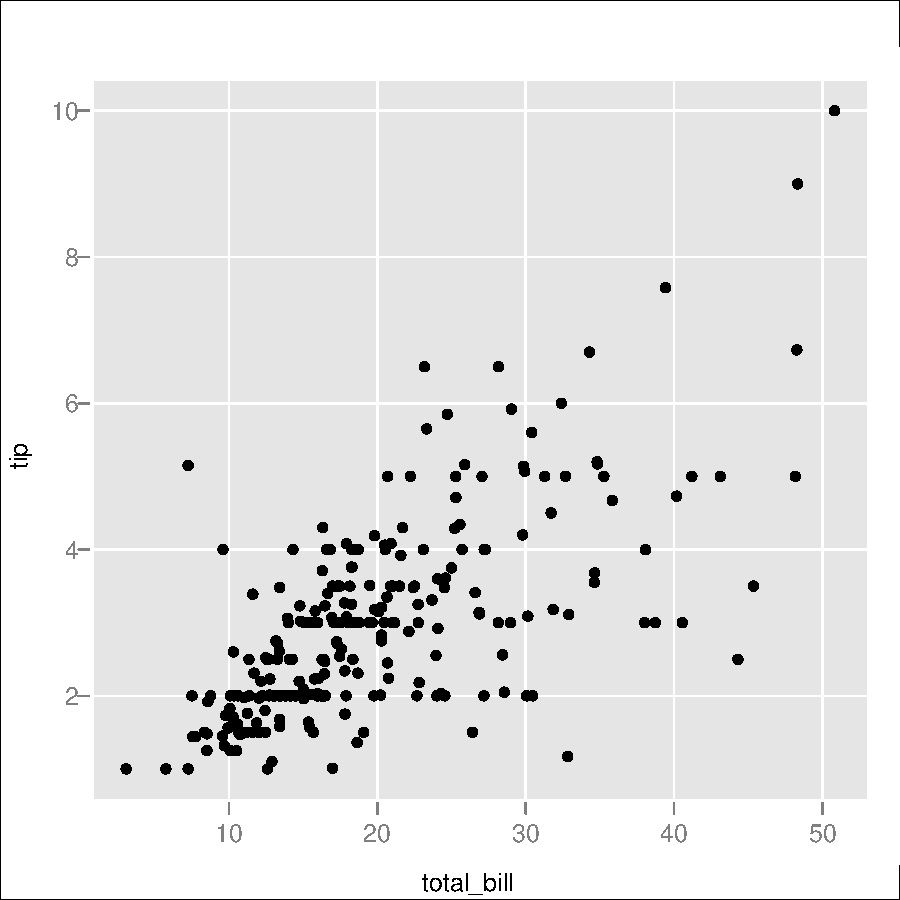
\includegraphics{introduction-003}

Let's investigate the difference between the sexes.  One way to do this is to display the sexes with different colours.  We can do this by adding an additional aesthetic mapping of colour to $sex$, as in this plot.  Note that a legend is automatically created for us.

\begin{Schunk}
\begin{Sinput}
> print(ggpoint(p, list(colour = sex)))
\end{Sinput}
\end{Schunk}
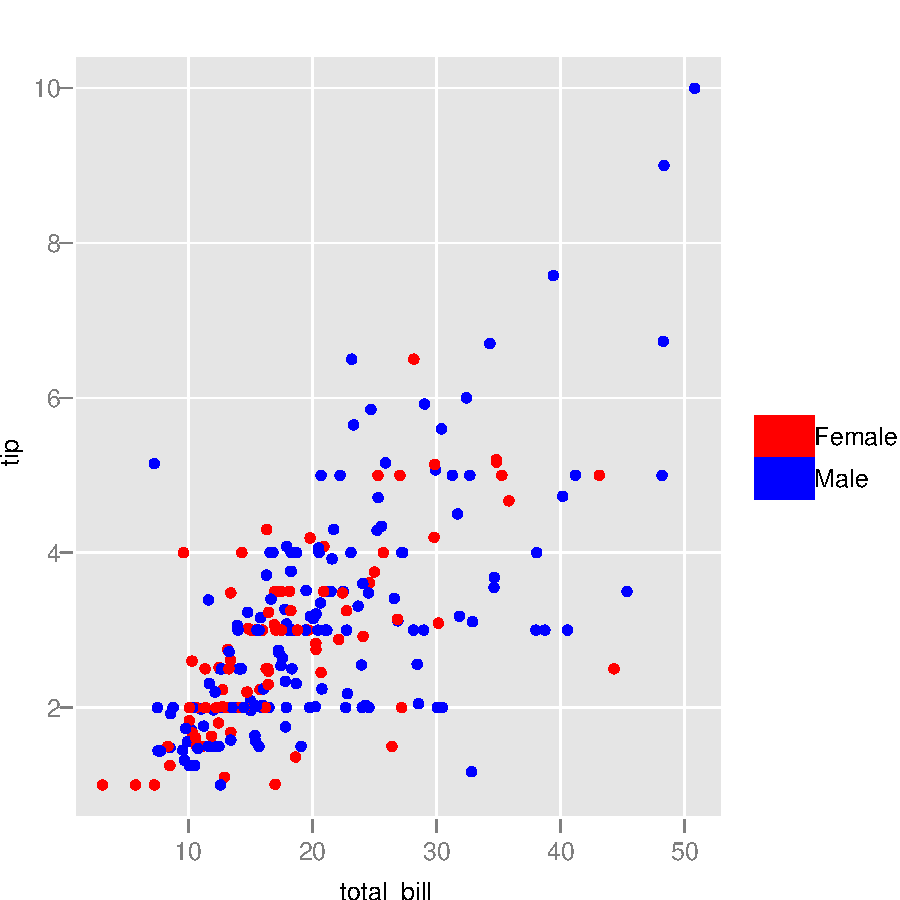
\includegraphics{introduction-004}

Another way to investigate the difference is to plot each sex on a different chart.  We can do this easily using facetting.  The facetting formula $. \sim sex$ says we don't want any facetting on the y-axis, but we want a separate plot for each sex arranged along the x-axis.

\begin{Schunk}
\begin{Sinput}
> print(ggpoint(ggplot(tips, . ~ sex, aesthetics = list(y = tip, 
+     x = total_bill))))
\end{Sinput}
\end{Schunk}
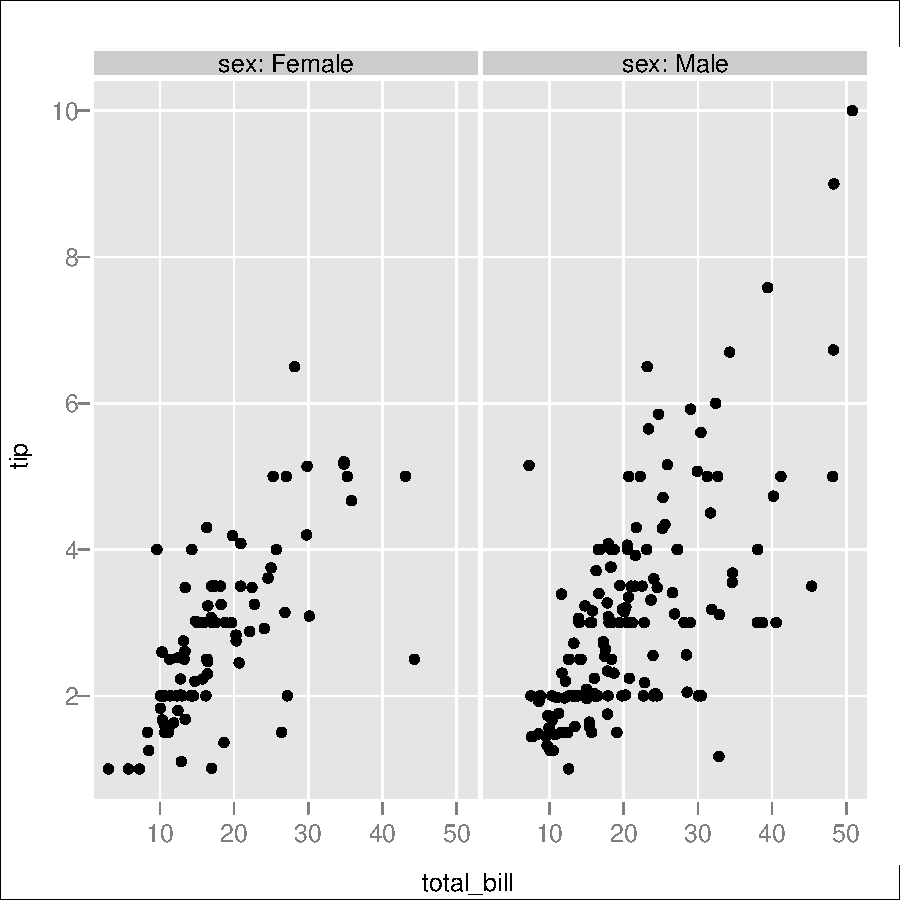
\includegraphics{introduction-005}

Similarly, if we want to explore the effect of smoking, we can add $smoker$ as an additional facetting variable on the $y$-axis.

\begin{Schunk}
\begin{Sinput}
> p <- ggplot(tips, smoker ~ sex, aesthetics = list(y = tip, x = total_bill))
> print(ggpoint(p))
\end{Sinput}
\end{Schunk}
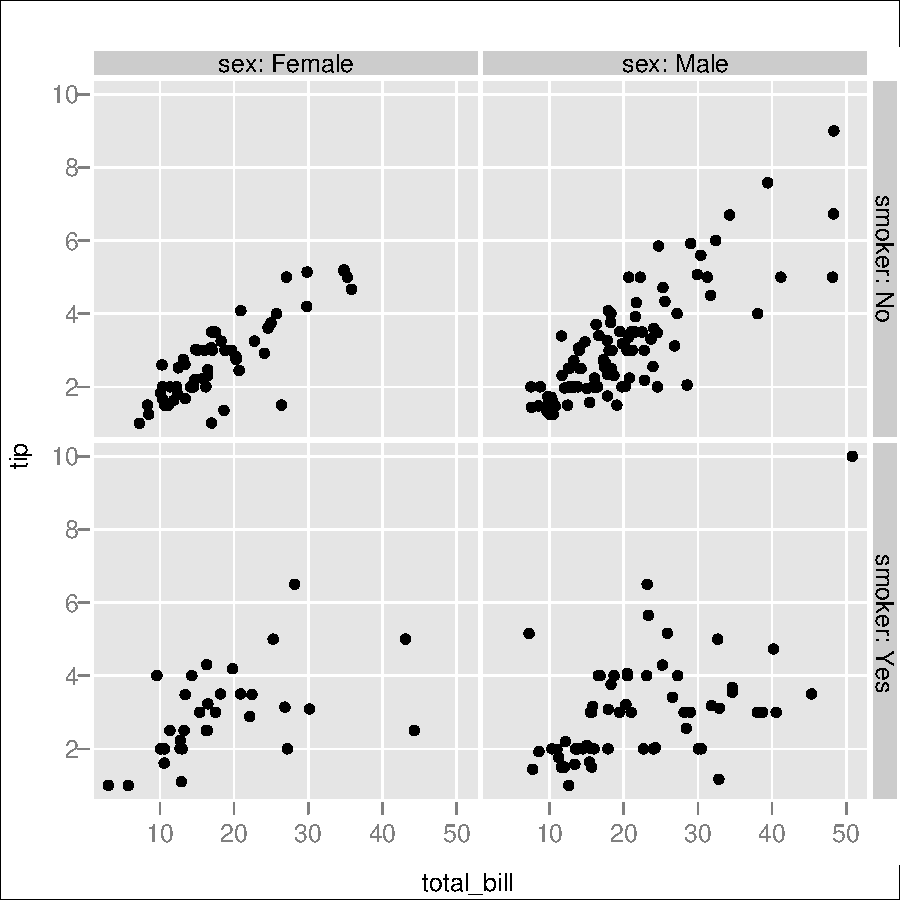
\includegraphics{introduction-006}

To make the differences easier to see, we might want to add a smoothed line.  In this example, we would expect the tip to be a constant proportion of the total bill, so a linear model would be appropriate.  The \texttt{smooth} grob adds a smooth line.  By default it uses \texttt{loess}, but we will tell it to use \texttt{lm} instead. 

\begin{Schunk}
\begin{Sinput}
> print(ggsmooth(ggpoint(p), method = lm))
\end{Sinput}
\end{Schunk}
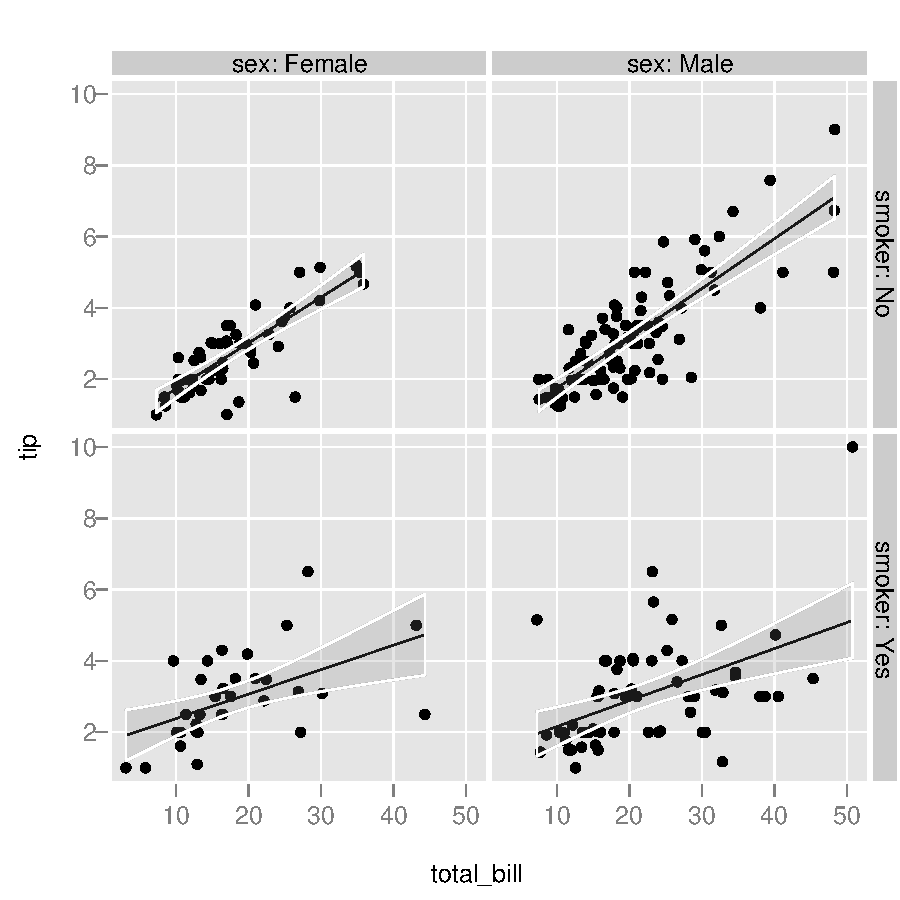
\includegraphics{introduction-007}

Another way of highlighting the difference between the plots is to add reference lines.  \texttt{ggabline} will add lines with specific intercept and slope, and here we add lines for $10\%$, $15\%$ and $20\%$ tips.

\begin{Schunk}
\begin{Sinput}
> print(ggabline(ggpoint(p), slope = c(0.1, 0.15, 0.2)))
\end{Sinput}
\end{Schunk}
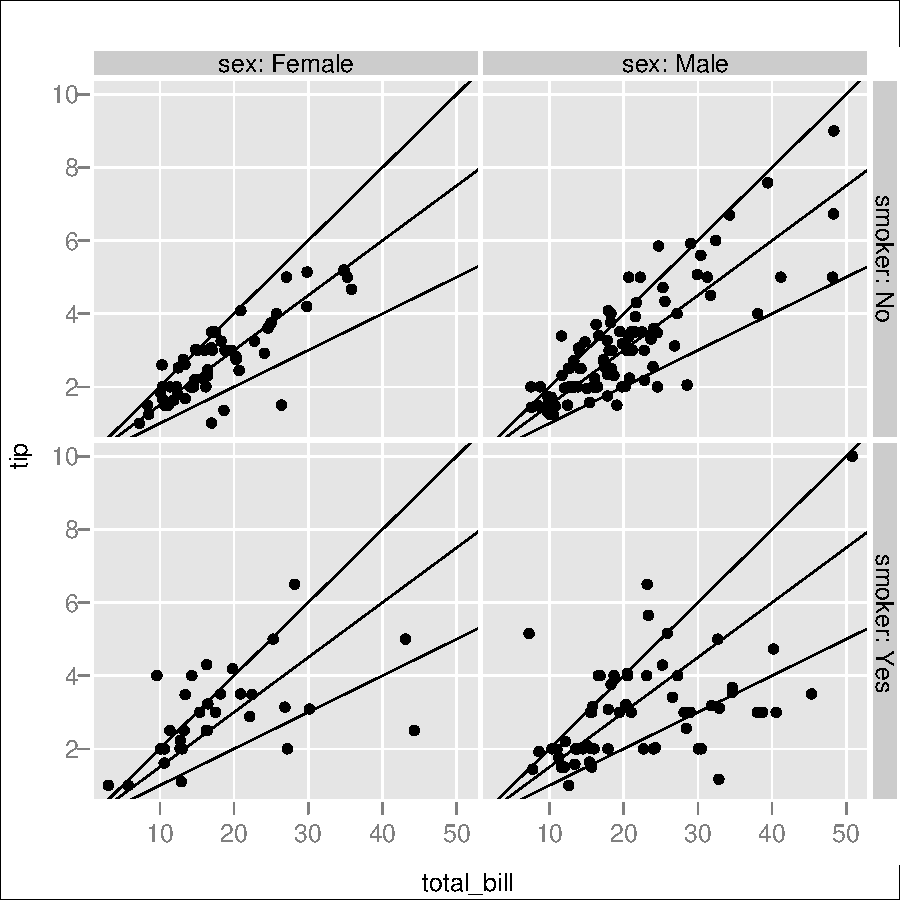
\includegraphics{introduction-008}

Finally, we can colour the points by the tip rate by mapping colour to $tip / total_bill$.  

\begin{Schunk}
\begin{Sinput}
> print(p2 <- ggabline(ggpoint(p, list(colour = tip/total_bill)), 
+     slope = c(0.1, 0.15, 0.2)))
\end{Sinput}
\end{Schunk}
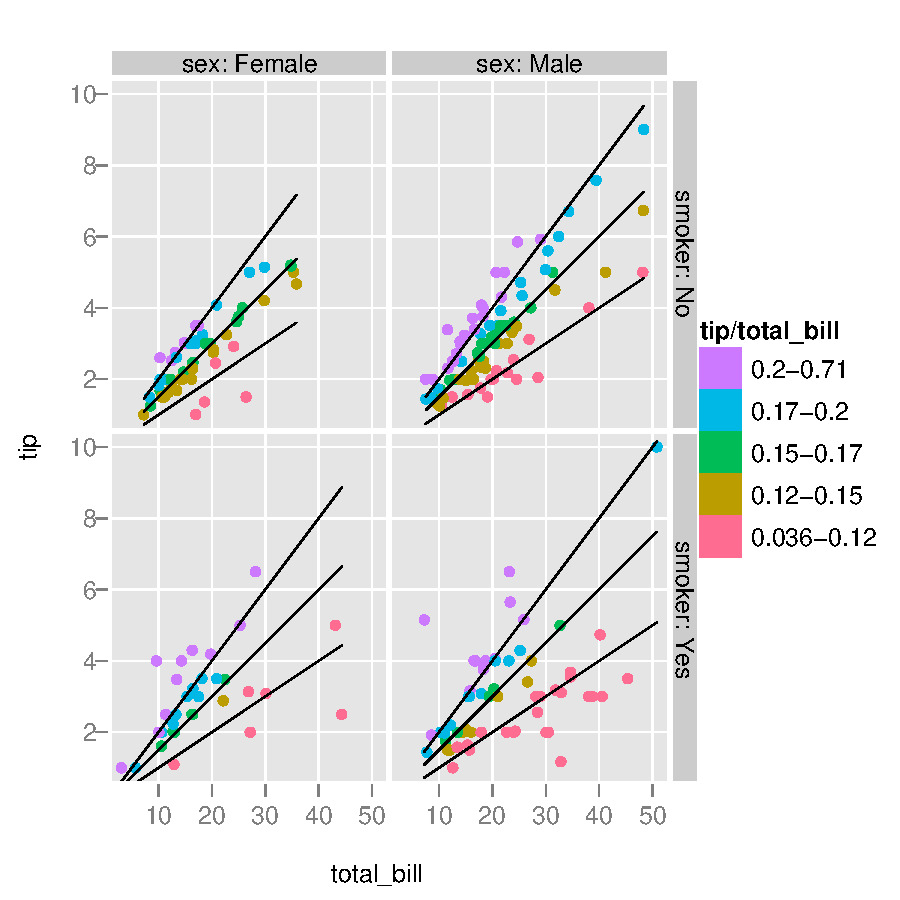
\includegraphics{introduction-009}

By default this does not use a very useful scale.  To remedy this, we add a new scale to the plot, \texttt{scgradient}, which produces a continuous colour gradient.  We will colour good tippers green, bad tippers red and those in the middle (those who tipped around $15\%$) yellow.  

\begin{Schunk}
\begin{Sinput}
> print(scgradient(p2, midpoint = 0.15, high = "green", mid = "yellow", 
+     low = "red"))
\end{Sinput}
\end{Schunk}
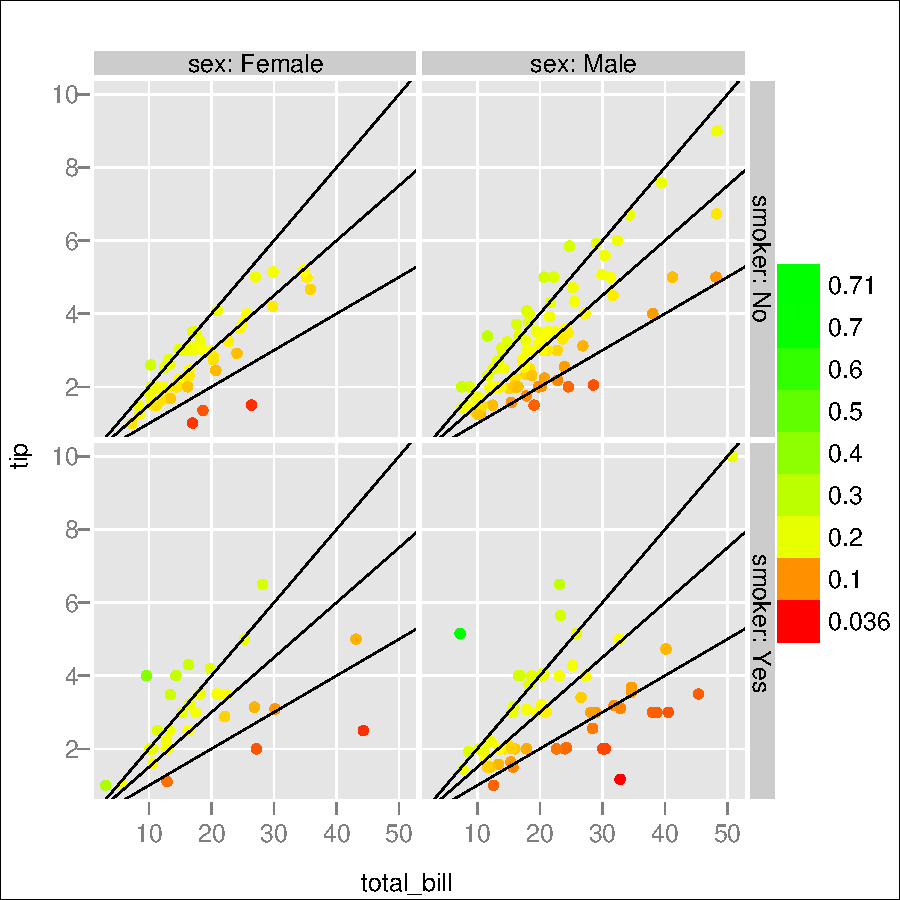
\includegraphics{introduction-010}

All scale functions start with \texttt{sc}, take a plot object and options, and then return the modified plot object with the new scale attached.  You can see a complete list of scales in \texttt{?ggplot}.

We can investigate the distribution of tip rates directly using a histogram.

\begin{Schunk}
\begin{Sinput}
> p <- ggplot(tips, sex ~ smoker, aesthetics = list(x = tip/total_bill))
> print(gghistogram(p, scale = "density"))
\end{Sinput}
\end{Schunk}

By default, the histogram will heuristically select the ``best'' number of bins in each facet.  This produces an undesirable effect in this example, so we will manually set the breaks to give a more pleasing graph.  This is an example of a parameter that controls the display of the grob.  See the help for individual grob functions for more details.

\begin{Schunk}
\begin{Sinput}
> print(gghistogram(p, scale = "density", breaks = seq(0, 1, length = 20)))
\end{Sinput}
\end{Schunk}
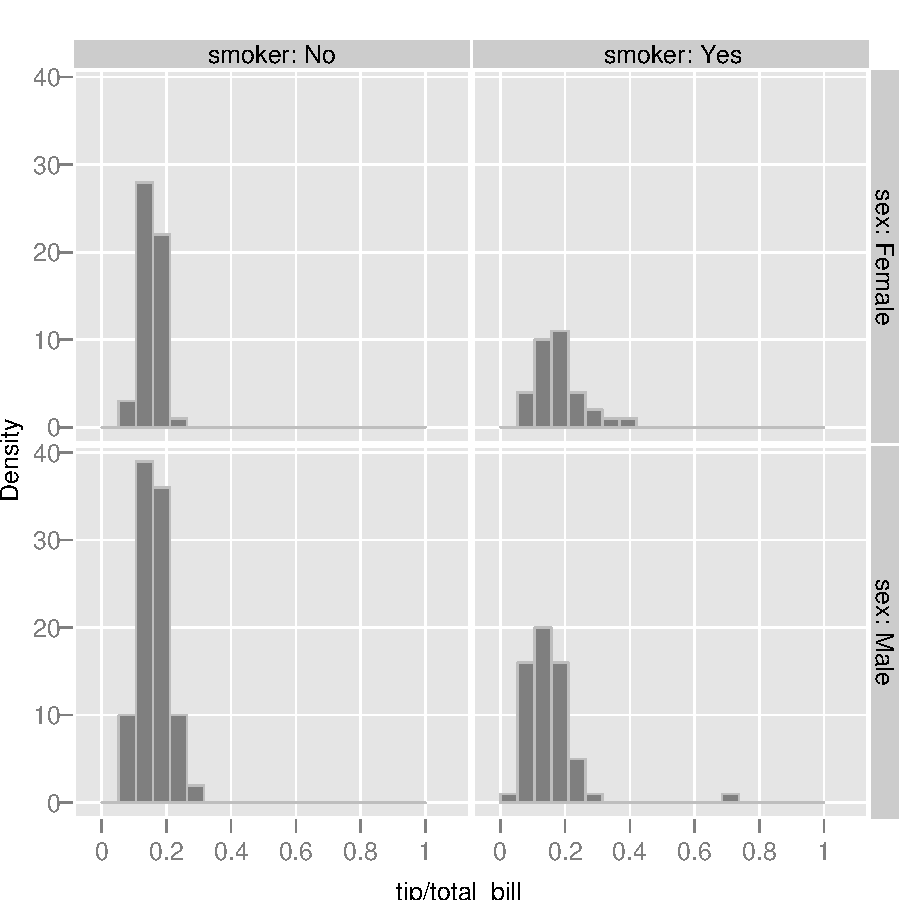
\includegraphics{introduction-012}

Finally, an example with boxplots:

\begin{Schunk}
\begin{Sinput}
> p <- ggplot(tips, . ~ smoker, aesthetics = list(x = sex, y = tip))
> print(ggboxplot(p))
\end{Sinput}
\end{Schunk}

If we want to see the actual points, we can overlay jitter points on top of the boxplot with \texttt{ggjitter}.  The jittering helps overcoming the overplotting problem associated with a categorical axis.

\begin{Schunk}
\begin{Sinput}
> print(ggboxplot(ggjitter(p)))
\end{Sinput}
\end{Schunk}
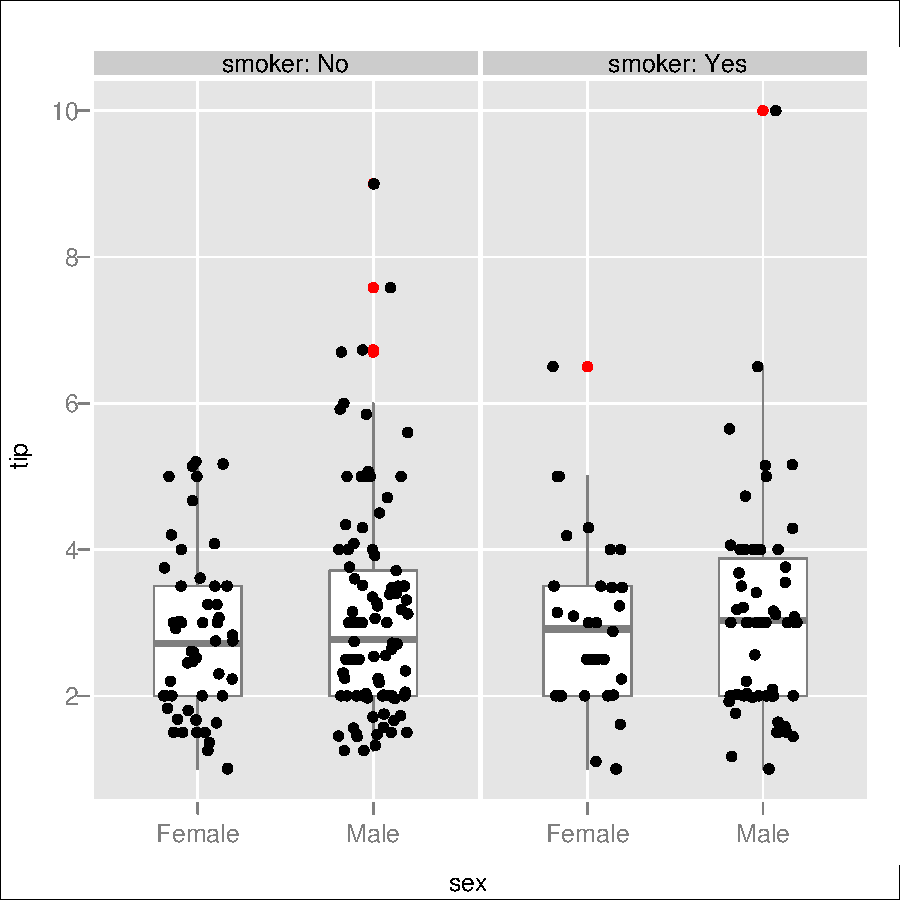
\includegraphics{introduction-014}

\section{Implementation}

The package, \texttt{ggplot}, is made up of a number of small independent building blocks.  This reduces redundancy within the code, and makes it easy to customise the graphic to get exactly what you want.  In rough order of complexity, the building blocks of \texttt{ggplot} are:

\begin{itemize}
	\item aesthetic mapping functions, which take data values and return aesthetics
	\item grob mapping functions, which take aesthetics and return grobs
	\item scale objects, which ensure mappings occur over a common domain, and produce guides for the plot
	\item the plot object, which brings the other pieces together
\end{itemize}

The \textbf{aesthetic maps} are simple functions that take one (or more) data attributes and return one (or more) vectors of aesthetics.  These are real numbers, integers, or strings depending on the particular aesthetic, e.g. numbers of size, integers for glyph types and strings for colour.  Some types of mapping can take both continuous and categorical vectors (eg. colour, size, rotation) while others can only accept categorical vectors (e.g. glyph, line type).  Position is also a type of aesthetic, and these maps correspond to scale transformations (e.g. log, power transform), where the axes are labelled on the original scale.

\textbf{Grob mapping functions} produce a list of grobs from a list of aesthetics and a number of optional parameters.  For example, the point grob function takes $x$ and $y$ coordinates, size, colour and glyph aesthetics and returns a points grob. Grob functions come in two varieties, simple and complex, and all start with \texttt{gg}.  Simple grob functions provide a common interface to the underlying grid functions for primitive graph types, eg. line, bar, point.  Complex grob functions, such as histograms or boxplots, will manipulate the data in some way before plotting.  They may also add new aesthetics mappings.  The histogram, for example, maps the number of points in each bin to the $y$ position. 

\textbf{Scale objects} are used when there are multiple panels in a plot, or multiple data sources on one panel.  They take data and a mapping function, and return a mapping function based on the common domain of the data.  For example, the $y$-axis needs to be shared across all panels in a row, and needs to be sufficiently wide to cover all the data points from different data sets.  Scales are responsible for producing the vector of aesthetics passed to the grob function.  Scales also provide function to produce guides: axes for position maps, and legends for the others.  Scales are added automatically to correspond to the aesthetic mappings you create.  If, however, you want to tweak the options of the scale you will need to manually add them. 

The \textbf{plot object} brings together these three components to make a plot.  It also stores a default data source, and breaks the plot down into the appropriate panels.  We can think of the plot function as performing a series of transformations from raw data to output grobs.  The first transformation normalises the names of the variables.  This is necessary when we have data sets with different variable names, and simplifies the job of the scale objects so that they can rely on a naming convention.  The second step is only performed by grobs that manipulate the data in some way before it is displayed, for example, the histogram grob.  After this step, the scale functions are run to work out what the mappings should be.  The fourth transformation then applies each scale function to the data to convert it from numbers to aesthetics.  The final step transforms these lists of aesthetics into grobs for plotting.

\section{Where to go next}

Now that you've read this introduction, you should be able to get started using \texttt{ggplot}.  I have tried to include lots of examples in the documentation, so if you get stuck have a look at those.  The best place to start is \texttt{ggplot} which includes links to all of the grob functions and scale objects.  If you write your own grob function, please see \texttt{vignette("writing-grob-functions")}.

If you have a problem and just can't figure out what's going wrong, please feel free to email me, \href{mailto:h.wickham@gmail.com}{h.wickham@gmail.com}.  I'd also love to hear your comments or any ideas that would make \texttt{ggplot} better.

\bibliographystyle{plain}
\bibliography{references}
\end{document}
